\documentclass[a4paper, 9pt]{article}
\usepackage{geometry}
%% % Geometry: es para modificar los márgenes del documento
\usepackage[left=3cm, right=2.5cm, top=2.5cm, bottom=2.5cm]{geometry}
%% lipsum: para generar texto de ejemplo. Se puede eliminar una vez que se eliminen todos los \lipsum[] del documento.
\usepackage{lipsum}
% lscape: en caso de querer rotar una hoja, buscar información en internet en caso de ser requerido. 
\usepackage{lscape}
\usepackage{float}
% inputenc: para que latex acepte caracteres latinos como los acentos y la letra ñ.
\usepackage[utf8]{inputenc}
% babel: para traducir los títulos que vienen originalmente en inglés. Ejemplo: Fecha, Chapter, Bibliography, Appendix, etc.
\usepackage[spanish,es-tabla]{babel}
% natbib: para poder citar utilizando paréntesis redondos con \citep{•} o sin parentesis con \cite{•}
\usepackage[numbers]{natbib}
\usepackage{float} % para usar [H] y obligar que las figuras o tablas aparezcan donde es requerido.
\usepackage[pdftex]{graphicx} % graphicx: para incorporar imágenes. Recordar que las imágenes 'gif' no son aceptadas por Latex, se sugiere utilizar formato png por su calidad, en segunda intantcia jpg.
\usepackage{parskip} % parskip: par no dejar sangrías e insertar espacios entre párrafos en su lugar.
\usepackage{amsmath} %paquete para escribir fórmulas matemáticas.
\usepackage{amsfonts}%paquete para escribir fórmulas matemáticas.
\usepackage{amssymb} %paquete para escribir fórmulas matemáticas.
\usepackage{amsbsy}
\usepackage{upgreek}
\usepackage[usenames,dvipsnames,svgnames,table]{xcolor} %xcolor: para definir colores y dar color a tablas.
\usepackage{multirow}

\graphicspath{ {figures/} }
\usepackage{array}

% hyperref: define opciones especiales para el documento PDF producido.
\usepackage[pdftex, bookmarksnumbered,  pagebackref, colorlinks=true, citecolor=DarkBlue, linkcolor=DarkBlue!30!Black, urlcolor=Black,bookmarksopen]{hyperref}

% El paquete fancyhdr es para definir opciones de encabezado y pié de página
% Según el formato existente a la fecha (agosto de 2015) esto no se considera
% Su utilización en este caso es para situar el número de página en la parte
% inferior derecha de la página.

\usepackage{fancyhdr} % activamos el paquete
	\pagestyle{fancy} % seleccionamos un estilo
	\lhead{} % texto izquierda de la cabecera
	\chead{} % texto centro de la cabecera
	\rhead{\textcolor[gray]{0.5}{\textit{\nouppercase \leftmark}}} % Nombre del capítulo. \nouppercase: uso de minúsculas
	\lfoot{} % texto izquierda del pie
	\cfoot{} % imagen centro del pie
	\rfoot{\textcolor[gray]{0.5}{\thepage}} % Número de página a la derecha, abajo
	\renewcommand{\headrulewidth}{0.2pt} % grosor de la línea de la cabecera

\fancypagestyle{detailed}{
    \fancyhf{} % clear all header and footers
    \fancyfoot[R]{\textcolor[gray]{0.5}{\thepage}}
	%\fancyhead{}    
    \renewcommand{\headrulewidth}{0pt}
 }
 
\usepackage{etoolbox}
\patchcmd{\chapter}{\thispagestyle{plain}}{\thispagestyle{detailed}}{}{}

%times: para uar letra tipo Times New Roman
\usepackage{times}

%separación entre líneas (1.2 espacios). En word es interlineado exacto a 12 pts
\renewcommand{\baselinestretch}{1.2} 

\usepackage{titlesec} % para poder modificar los títulos

% Para la numeración de tablas y figuras.
\renewcommand\thefigure{\arabic{section}.\arabic{figure}} % Genera numeración X.Y
\renewcommand\thetable{\arabic{section}.\arabic{table}} % Genera numeración X.Y
\numberwithin{figure}{section} %Hace que la primera figura de cada sección X sea X.1
\numberwithin{table}{section} %Hace que la primera tabla de cada sección X sea X

\usepackage{booktabs} % Para trabajar con opciones especiales de tablas.
\usepackage{caption}

\usepackage{setspace}

% El índice de tablas e imágenes se superpone el texto al número de la figura o tabla.
% Esta configuración arregla dicho problema, modificar el 3.0 de ser necesario.
\usepackage{tocloft}
\addtolength{\cftfignumwidth}{3.0em}
\renewcommand{\cftfigpresnum}{\figurename\ }
\addtolength{\cfttabnumwidth}{3.0em}
\renewcommand{\cfttabpresnum}{\tablename\ }
\usepackage[utf8]{inputenc}
\usepackage{amssymb}
\usepackage{graphicx}
\usepackage{lscape}
\usepackage{float}
\usepackage{changepage}
\usepackage{capt-of}
\usepackage{wrapfig}

\begin{document}

\begin{titlepage}
		\begin{center}
		\vspace{5 mm}\textbf{\Large UNIVERSIDAD POLITÉCNICA DE MADRID} \par
		\vspace{10 mm}
      			\begin{figure}[htb]
				\begin{center}
					
\includegraphics[scale=0.3]{./images/logo-upm.eps}
				\end{center}
			\end{figure}\par
  
      %\vspace{10 mm}\textbf{\large \degree} \par
      %\vspace{10 mm}\textbf{\large \faculty} \par
      %\vspace{20 mm}\textbf{\large \department } \par


      \vspace{20 mm}\textsc{\Large Homework 1.1 \\ Análisis del conjunto de datos de \\ enfermedades coronarias en Sudáfrica } \par
      
      \vspace{10 mm}\textsc{STATISTICAL DATA ANALYSIS}\par
      \vspace{10 mm}\textsc{AUTORES: \\ Cristian Abrante Dorta, \\ Álvaro Arranz Domínguez, \\ Ángel González López, \\ Daniel Saiz González}\par
		
	\rule{80mm}{0.1mm}\\      
      
	  \vspace{10 mm}
      \textsc{Master's Programme in ICT Innovation: Data Science}\par 
      %\vfill\textrm{\address. \hfill \monthyear}
      
      
      \vspace{10 mm}\textsc{ESCUELA TÉCNICA SUPERIOR DE INGENIERÍA DE INFORMÁTICA}		
		\end{center}
\end{titlepage}


\newgeometry{textwidth=18cm,textheight=27cm}

\section{Descripción del conjunto de datos}
\label{sec:descripcion-datos}
\noindent

Este conjunto de datos es una muestra retrospectiva de hombres en una región de alto riesgo de enfermedad cardiaca de Cabo Occidental, Sudáfrica. Muchos de los hombres con cardiopatía coronaria positiva se han sometido a un tratamiento de reducción de la presión arterial y a otros programas para reducir sus factores de riesgo después del evento de cardiopatía coronaria. En algunos casos, las mediciones se hicieron después de estos tratamientos. Estos datos se han tomado de un conjunto de datos más amplio descrito en Rossouw et al (1983) Coronary risk factor screening in three rural communities, South African Medical Journal.

\subsection{Descripción de las variables de estudio}
Las variables de estudio que se encuentran representadas en el dataset son las siguientes:

\begin{itemize}
    \item \texttt{cbp}: Presión arterial sistólica.
    \item \texttt{ldl}: nivel de lipoproteínas de baja densidad (colesterol).
    \item \texttt{adiposity}: acumulación o exceso de grasa en el cuerpo.
    \item \texttt{typea}: El comportamiento de tipo A es una medida psicológica que se aplica a las personas con carácter hiperactivo e impaciente, o que se someten a altos niveles de estrés. La escala de medida se establece a partir del test de escala corta de Bortner \cite{bortner1969short}, variando entre los valores: 12 y 84.
    \item \texttt{obesity}
    \item \texttt{Alcohol}: consumo actual de alcohol.
    \item \texttt{age}: Edad.
    \item \texttt{chd}: Si padece o no una enfermedad coronaria.
\end{itemize}

\section{Preguntas de investigación}
\noindent
El objetivo de esta investigación es dar respuesta al conjunto de preguntas formuladas aplicando diferentes técnicas de visualización y transformación de datos.


\subsection{¿Tener un historial familiar de cardiopatía coronaria afecta la posibilidad de que un paciente tenga cardiopatía coronaria? ¿Este resultado cambia para los pacientes menores de \texttt{40} años de edad? ¿Qué pasa con los pacientes de \texttt{40} años o más?}

\vspace{3mm} 

La preparación de los datos fue simple. Se estudiaron que campos iban a ser clave para resolver esta pregunta, los cuales erán \texttt{famhist} y \texttt{chd}. Al ser dos variables categóricas, es decir, que solo pueden tomar valores dentro de un conjunto, lo que se hizo fue convertir ambos datos a Factor. Para poder mostrar mejor los plots que se fueran a utilizar. Para la investigación se ha utilizado el Diagrama de Barras (\emph{Bar Plot}) para la primera pregunta e Histogramas (\emph{Histogram Plot}) para las siguientes. Por ello, para empezar se ha analizado el numero de datos por cada variable, tanto en \texttt{famhist} como en \texttt{chd}. 

\begin{wrapfigure}{r}{0.3\linewidth}
    \centering
    \begin{tabular}{|c||c|c|}
        \hline
          & Absent & Present   \\ \hline \hline
        0 & 0.6821192 & 0.3178808 \\ \hline
        1 & 0.4000000 & 0.6000000 \\ \hline
    \end{tabular}
    \label{tabla:question1-porcentagetable}
\end{wrapfigure}

Teniendo como resultado \textbf{302} pacientes que padecen una enfermedad coronaria y \textbf{160} pacientes que no; y \textbf{270} pacientes que poseen un historial con familiares que han padecido enfermedad coronaria y \textbf{192} pacientes que no. Lo siguiente que se ha realizado es evaluar cuantos pacientes con y sin una enfermedad coronaria hay dentro del grupo de pacientes que tienen o no un historial de familiares que han padecido esta enfermedad. Teniendo como resultado un diagrama de barras que hemos traducido en la siguiente tabla de porcentajes:

\vspace{3mm} 

Con estos datos, podemos decir con certeza que el hecho de poseer familiares que han padecido esta enfermedad incrementa las posibilidades, casi en el doble, de padecer la enfermedad coronaria. Como podemos observar con la ayuda de los porcentajes de la tabla \ref{tabla:question1-porcentagetable}, los pacientes que tienen historial familiar suponen un 60\% de los que tienen dicha enfermedad, mientras que los que no tienen historial familiar solo suponen un 31,79\% de los pacientes sin enfermedad. Por ello, desde una visión general podemos afirmar el impacto del historial familiar con las posibilidades de padecer una enfermedad coronaria.

\vspace{3mm}

\begin{wrapfigure}{r}{0.3\linewidth}
    \centering
    \begin{subfigure}
        \centering
        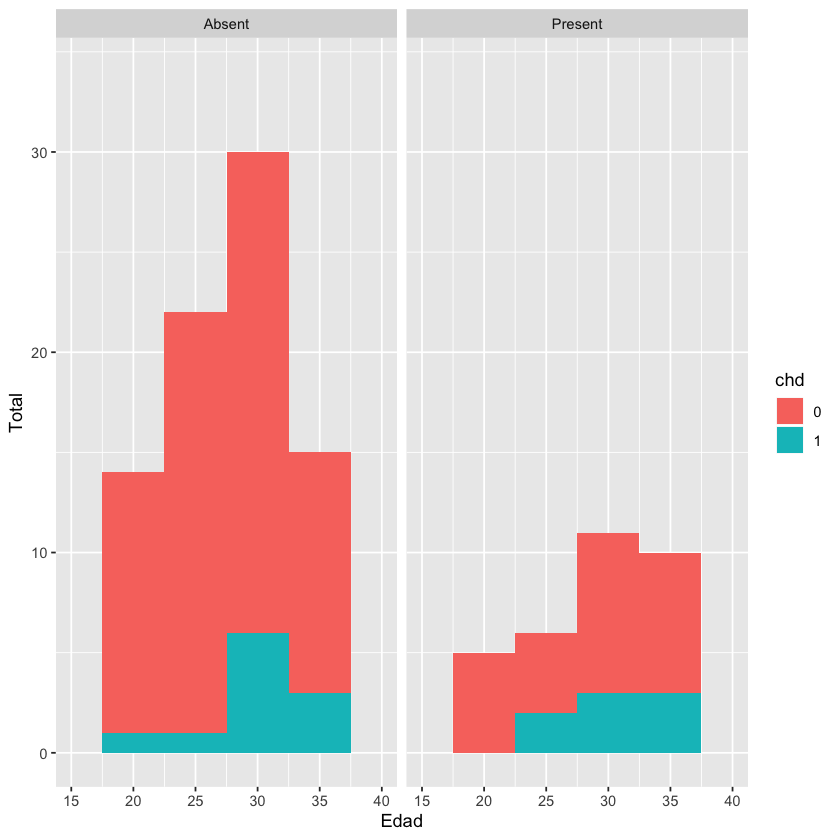
\includegraphics[scale=0.15]{images/question-1/histogram_less40.png}
        \label{image:question1-histogram_less40}
    \end{subfigure}
    \begin{subfigure}
        \centering
        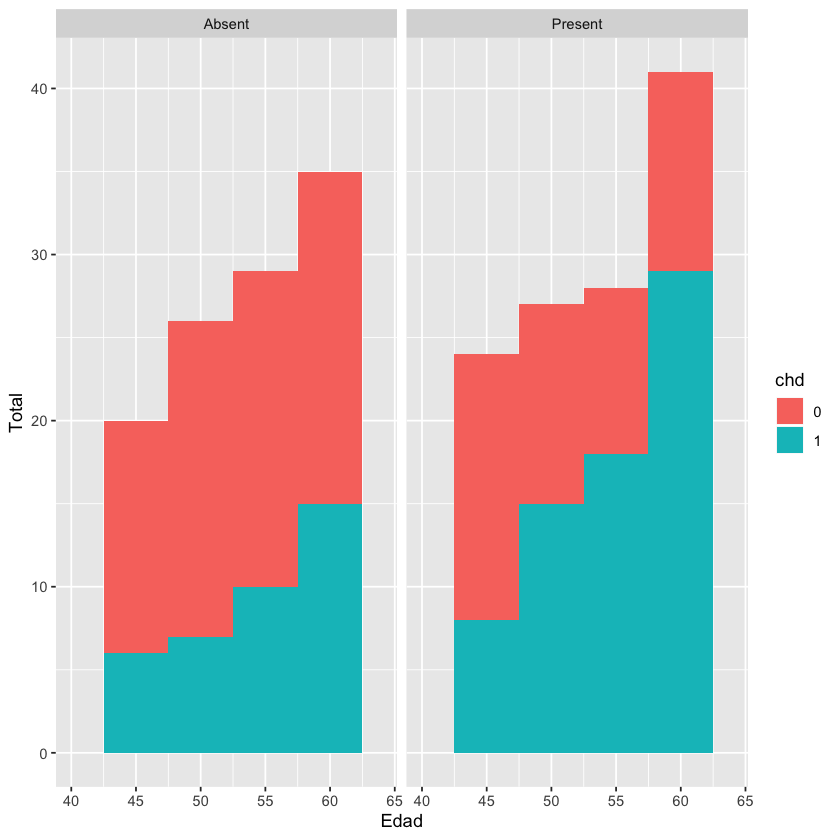
\includegraphics[scale=0.15]{images/question-1/histogram_more40.png}
        \label{image:question1-histogram_more40}
    \end{subfigure}
\end{wrapfigure}

\vspace{3mm}

A continuación, se estudiará lo mismo dentro del sesgo de pacientes con menos de 40 años. Para ello, lo que hemos hecho es utilizar dos histogramas, uno con los pacientes que poseen historial familiar y otro con los que no. Dentro de esta separación hemos hecho un sesgo, habiendo analizado previamente cual era el mínimo de edad dentro del dataset. Por ello, los datos que vemos dentro de la \textit{\textbf{Figura 2 a la izquierda}} son los relativos a los pacientes comprendidos entre los \texttt{15} años y los \texttt{40} años. En el diagrama antes mencionado, no vemos tan clara la diferencia entre ambos grupos de pacientes como observábamos en el diagrama de barras. Por ello, podemos decir que el resultado de la pregunta anterior cambia radicalmente, ya que en estos grupos no podemos ver ninguna diferencia notable entre ambos. Si basásemos el estudio en este grupo de pacientes concluiríamos que no existe dicha diferencia y que por lo tanto, el dato del historial familiar no es clave dentro de las posibilidades de tener o no enfermedades coronarias.

\vspace{3mm}

A continuación, se estudiará lo mismo dentro del sesgo de pacientes con más de 40 años. Utilizando la misma táctica del anterior diagrama y, también, habiendo analizado previamente cual era el máximo de edad dentro del dataset. Por ello, los datos que vemos dentro de la \textit{\textbf{Figura 2 a la derecha}} son los relativos a los pacientes comprendidos entre los \texttt{40} años y los \texttt{64} años. Si en la primera pregunta veíamos una diferencia entre ambos grupos y en la segunda dicha diferencia desaparecía, con este histograma vemos de forma muy notable la diferencia que comentábamos entre los grupos en la primera pregunta.

\vspace{3mm}

\setcounter{figure}{0}
\setcounter{table}{0}

\subsection{Explorar la relación entre los niveles de \texttt{LDL} y las variables categóricas del conjunto de datos}

Observando el conjunto de datos, solamente se encuentran dos variables cuyo tipo es categórico: \texttt{famhist}, que explica si existe herencia familiar de enfermedades del corazón y \texttt{chd} que representa si el paciente posee una enfermedad coronaria.

\begin{table}[H]
\centering
\begin{tabular}{c|cc}
                  & \texttt{famhist} = Absent & \texttt{famhist} = Absent  \\ \hline
\texttt{chd} = 0  & 00               & 01                \\
\texttt{chd} = 1  & 10               & 11               
\end{tabular}
\label{table:question2-combinations}
\end{table}

\begin{wrapfigure}{r}{0.4\linewidth}
    \centering
    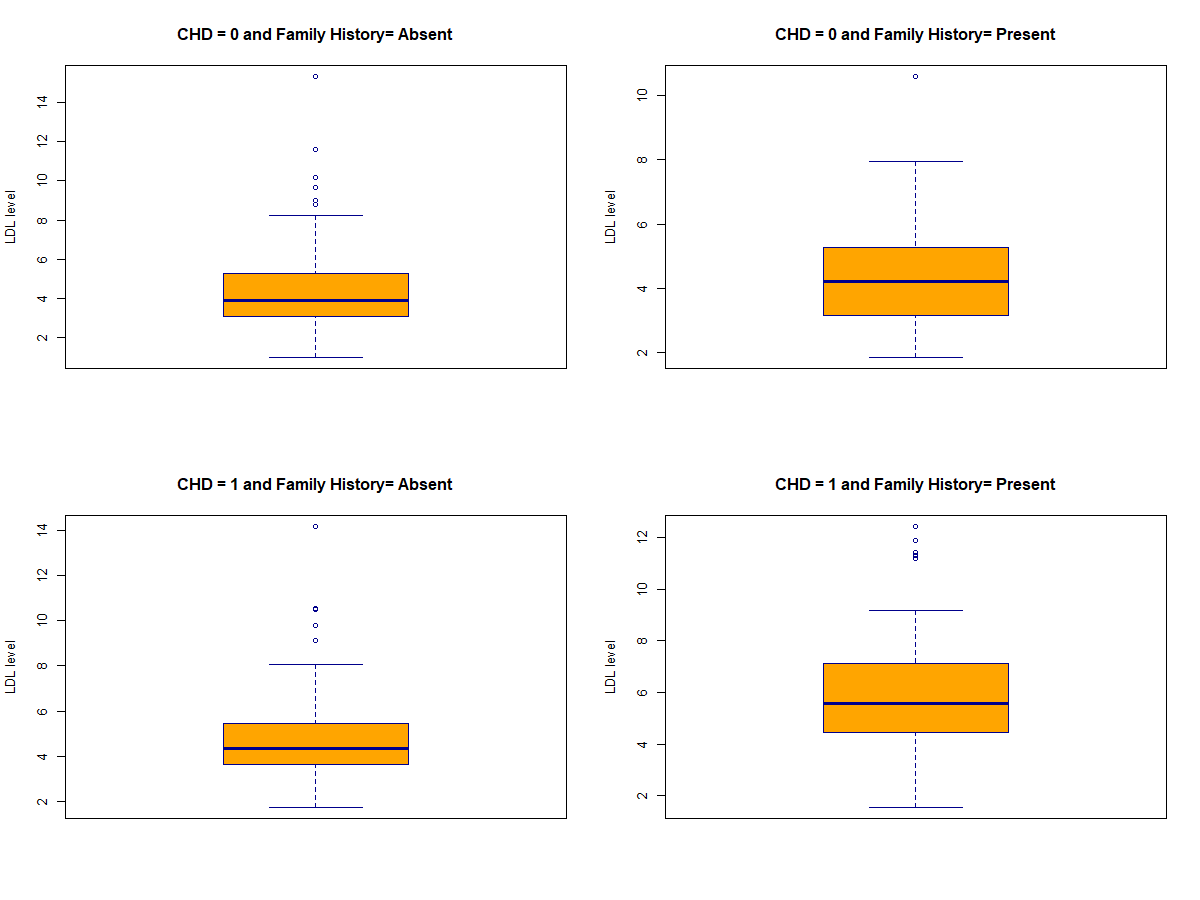
\includegraphics[scale=0.2]{images/question-2/plot1.png}
    \label{fig:question2-plot}
\end{wrapfigure}


La primera variable, se representa en el conjunto de datos como \textit{Present} o \textit{Absent}, en el caso en el que haya o no herencia familiar, respectivamente. Sin embargo, en el segundo caso, las dos opciones posibles que toma la variable son 0 y 1 en el caso que exista o no una afección coronaria. En este caso, por defecto, son detectados como números enteros, por lo que la variable chd es considerada como continua. Para lograr que sea categórica, se indica que los dos únicos factores que puede tomar la variable \textit{chd} son 0 y 1, por lo que a partir de este momento sí que sería una variable categórica. Para poder detectar mejor las diferencias en los niveles de LDL según la historia familiar y la presencia de patologías coronarias, se van a combinar las dos variables categóricas que son objeto de estudio en esta pregunta. Se obtienen de esta forma 4 combinaciones posibles, como se describe en la tabla \ref{table:question2-combinations}.

\vspace{3mm}

Tal y como se puede observar en los diferentes diagramas de caja y bigotes de la figura 3, para cada una de las situaciones anteriormente planteadas, los niveles medios de LDL son diferentes para cada caso, así como su desviación típica y los cuartiles, como se puede ver en la figura \ref{fig:question2-plot}. 

\begin{table}[H]
\centering
\begin{tabular}{c|c|c|cl}
Caso & Media aritmética & Desviación típica & Cuartil 75\% &  \\ \cline{1-4}
00   & 4.31             & 1.96              & 5.26         &  \\
01   & 4.4              & 1.66              & 5.28         &  \\
10   & 4.92             & 2.19              & 5.45         &  \\
11   & 5.87             & 2.18              & 7.08         & 
\end{tabular}
\caption{Estudio estadístico de los valores de \textit{LDL} según cada caso}
\end{table}

En los casos en los que no se tiene historia familiar (Absent) no se producen grandes diferencias entre los niveles de LDL se tenga o no una afección coronaria. Pero, sin embargo, si se cuenta con antecedentes familiares (Present), los niveles de LDL son ligeramente mayores, independientemente de si cuenta con alguna patología. Esto, indica que los niveles de LDL tienen una fuerte relación con los antecedentes familiares y, en menor medida, con la presencia de enfermedades coronarias.
El aumento de la desviación típica guarda relación la aparición de patologías y de antecedentes familiares. Una persona sana y sin historia (caso 00) tendrá valores de LDL más normales, y es más extraño que se tengan valores mucho más altos de los valores normales para una persona sana, porque eso conllevaría la aparición de alguna enfermedad o de algún factor. Sin embargo, para pacientes enfermos y con antecedentes (caso 11) es más común que existan valores más atípicos (pacientes enfermos cuyos niveles siguen siendo muy altos). Finalmente, se observa mayor diferencia entre los niveles de LDL del caso 11 con el resto en el cuartil 75\%. Se hace en este y no en el 25\% ya que, si un nivel es atípico, lo será generalmente porque es mayor y no menor que la media.


\subsection{Explorar la relación entre los niveles de \textit{LDL} y atributos como el tabaco, la obesidad, la adiposidad y el alcohol.} \label{sssec:ldltobaccoalcoholobesityadiposity}

\vspace{3mm}

Al tratarse de variables numéricas continuas, hemos decidido usar
diagramas de dispersión. Primero hemos comparado cada una de las variables con el \texttt{ldl} (o
coloresterol malo)

\begin{figure}[ht]
    \centering
    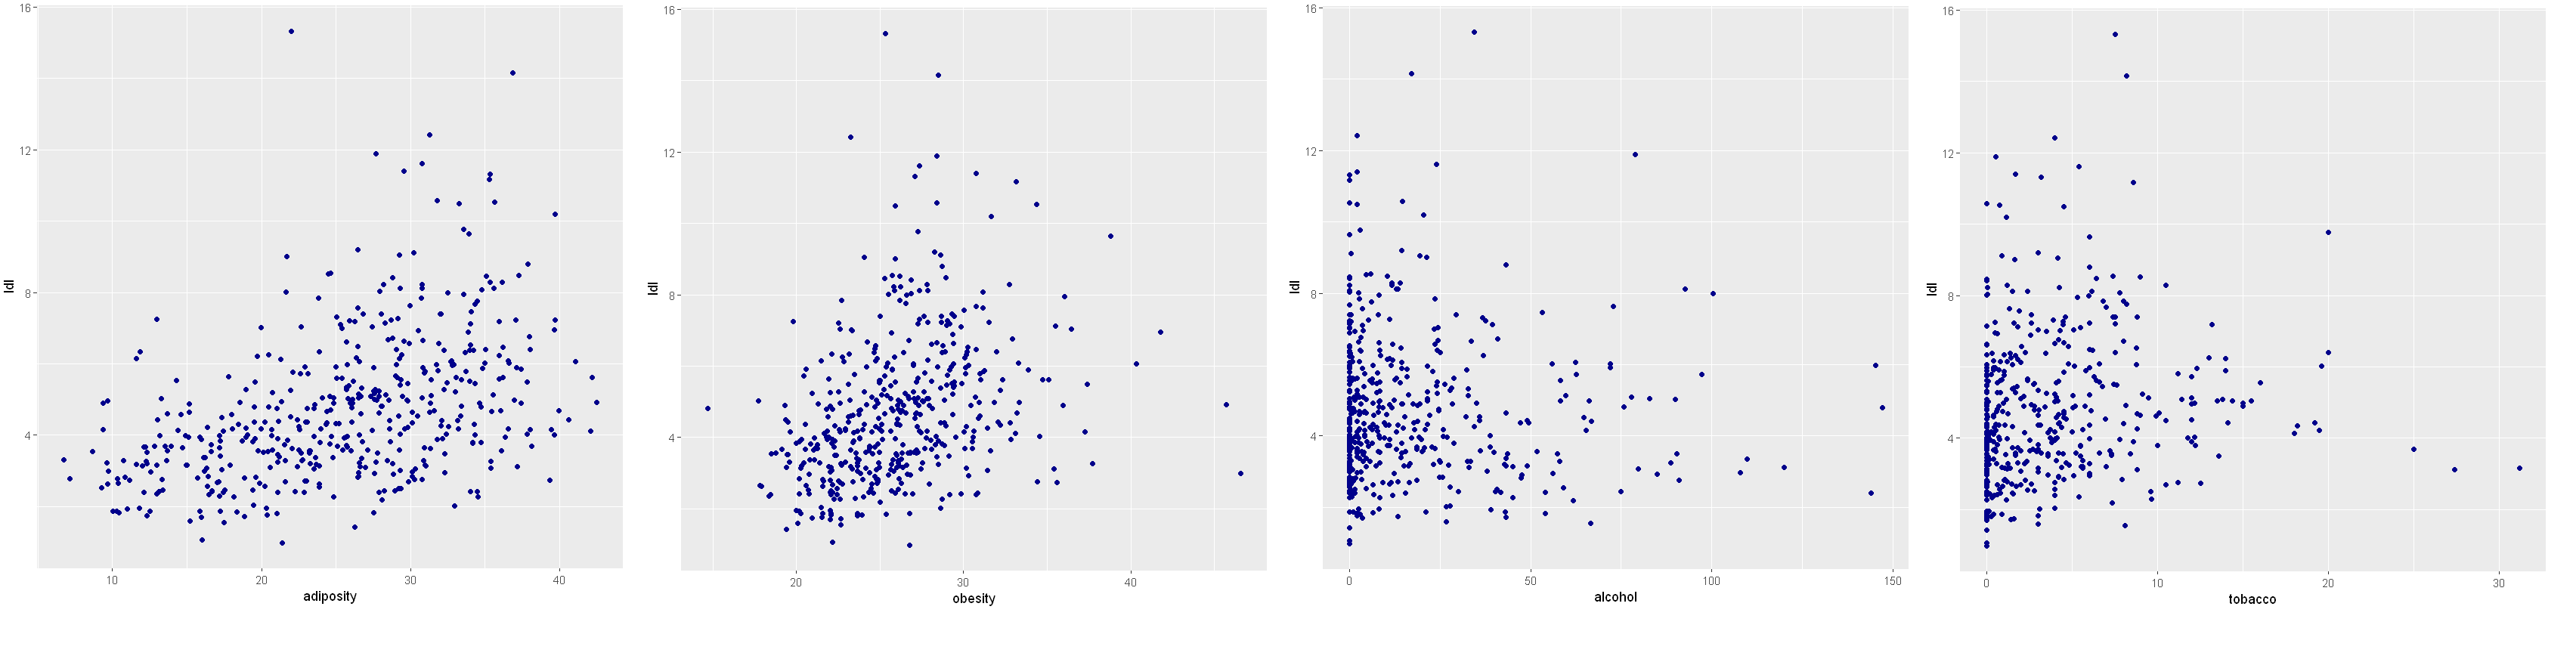
\includegraphics[scale=0.20]{images/question-3/ldlvsvariables.png}
    \caption{Relación entre \textbf{obesidad}, \textbf{adiposidad} y \textbf{ldl}}
    \label{fig:scatteralcoholtobacco}
\end{figure}

\begin{wrapfigure}{r}{0.50\linewidth}
    \centering
    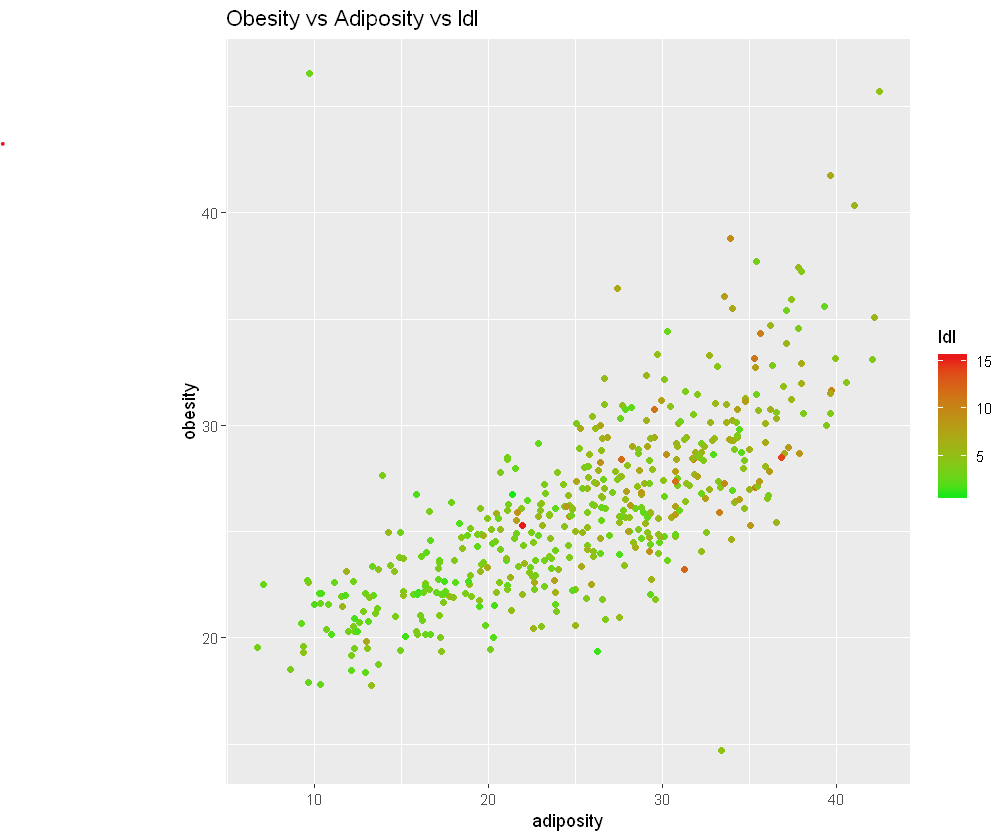
\includegraphics[scale=0.36]{images/question-3/obsityvsadiposityvsldl.png}
    \caption{Relación entre \textbf{obesidad}, \textbf{adiposidad} y \textbf{ldl}}
    \label{fig:obsityvsadiposityvsldl}
\end{wrapfigure}

Si estudiamos la relación entre los niveles de \texttt{ldl} y \texttt{obesity} en la gráfica 2 de la figura 1 vemos una ligera correlación. Esta relación se hace más visible si comparamos \texttt{ldl} y \texttt{adiposity}, (en la gráfica 1) teniendo en este caso una pendiente más ligera.


Las gráficas 3 y 4 de la figura 1, que muestran la comparación de las variables \texttt{tobacco} y \texttt{alcohol} con la variable \texttt{ldl}, son  similares sin reflejar ninguna ninguna relación relevante con los niveles de \texttt{ldl}. Afirmamos esto por el amplio rango de valores que toma \texttt{ldl} para niveles bajos de consumo de ambas sustancias (cercanos a 0), y no parece haber una tendencia clara de los niveles de colesterol malo se incrementa el consumo. 

\vspace{3mm}

En la figura \ref{fig:obsityvsadiposityvsldl} comparamos \texttt{obesity} con los niveles de \texttt{adiposity} y observamos que según aumentan los niveles de adiposidad, aumentan los de obesidad. Ambas variables son comparadas con los niveles de colesterol malo y observamos como en valores bajos de las dos variables (por debajo de 25 en obesidad y 20 adiposidad) se encuentran los valores más bajos de ldl.

\vspace{3mm}

\setcounter{figure}{0}
\setcounter{table}{0}

\subsection{Analizar la variable \texttt{tipea}, estableciendo la relación con la presencia de la enfermedad coronaria}

Tal y como se ha comentando, la variable \texttt{typea}, sirve para medir en una escala numérica ordinal el nivel de comportamiento tipo A que presenta el individuo. En diversas investigaciones, el valor en esta escala se ha relacionado con la presencia de enfermedades cardiacas, relación que intentaremos corroborar para nuestro conjunto de datos. Además de esto, sería interesante comprobar si esta relación se establece de igual manera a todas las edades.

\vspace{3mm}

Para establecer esta relación, deberemos llevar a cabo una serie de transformaciones en el conjunto de datos. En primer lugar, debemos categorizar la variable \texttt{chd}, de tal forma que deje de tener un valor numérico y asignarle la etiqueta \texttt{Present} o \texttt{Absent}. A continuación, crearemos una variable adicional que determina si la variable \texttt{typea} está por encima del \textbf{valor 55}, el considerado por Rossouw y Du Plessis como el umbral de comportamiento. Finalmente, con el objetivo de ver de una manera más clara los grupos de edades, se han reorganizado en los siguientes intervalos: entre 0 y 25 años, entre 26 y 35 años, entre 36 y 55 años y mayores de 55 años. Una vez que hemos preparado el conjunto de datos, establecemos una relación mediante este gráfico:

\vspace{3mm}

\begin{figure}[H]
    \centering
    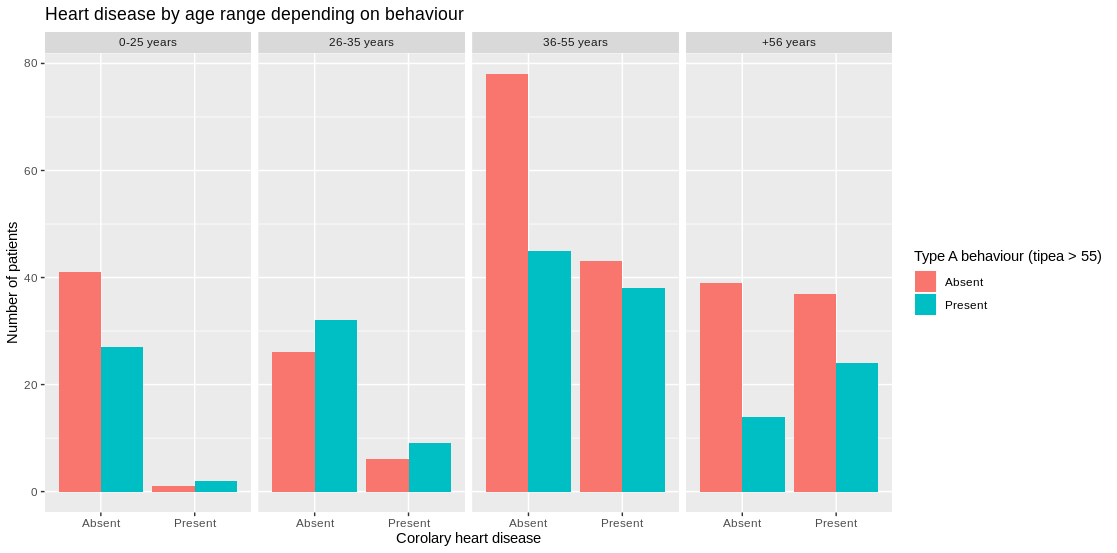
\includegraphics[scale=0.31]{images/question-4/plot1.png}
    \caption{Relación entre el \textbf{rango de edad}, \texttt{enfermedad coronaria} y \textbf{comportamiento de tipo A categorizado}}
    \label{fig:question4-uplot1}
\end{figure}

\vspace{3mm}

Este gráfico de barras establece las relaciones entre las variables por rango de edad. Para un mejor análisis debemos describir el histograma de frecuencias por cada rango. Es importante destacar que se ha excluido el rango de edad entre 0 y 25 años porque casi no existen casos que presenten la enfermedad, por lo que no lo consideramos relevante para este estudio.
    \begin{table}[!htb]
        \centering
        \begin{tabular}{ll}
        \begin{tabular}{c|c|c|c|}
        \cline{2-4}
                                                           & Con Tipo A     & Sin Tipo A     & Suma \\ \hline
        \multicolumn{1}{|c|}{Con chd}     & 9                          & 6                          & 15   \\ \hline
        \multicolumn{1}{|c|}{Sin chd}     & 32                         & 26                         & 58   \\ \hline
        \multicolumn{1}{|c|}{Suma}                         & 41                         & 32                         & 73   \\ \hline
        \end{tabular}
        &
        \begin{tabular}{c|c|c|c|}
            \cline{2-4}
                                                           & Con Tipo A    & Sin Tipo A      & Suma \\ \hline
        \multicolumn{1}{|c|}{Con chd}     & 38                         & 43                         & 81   \\ \hline
        \multicolumn{1}{|c|}{Sin chd}     & 45                         & 78                         & 123   \\ \hline
        \multicolumn{1}{|c|}{Suma}                         & 83                         & 121                        & 204   \\ \hline
        \end{tabular}
        \end{tabular}
    \end{table}
    
    \begin{table}[!htb]
        \centering
        \begin{tabular}{c|c|c|c|}
        \cline{2-4}
                                                       & Tipo A $\geq$ 55     & Tipo A \textless{} 55      & Suma \\ \hline
        \multicolumn{1}{|c|}{Con chd}     & 24                         & 37                         & 61   \\ \hline
        \multicolumn{1}{|c|}{Sin chd}     & 14                         & 39                         & 53   \\ \hline
        \multicolumn{1}{|c|}{Suma}                         & 38                         & 76                         & 114   \\ \hline
        \end{tabular}
        \caption{Tabla de frecuencias para diferentes rangos de edad: de 25 a 35 años, de 36 a 55 años y más de 55 años}
        \label{tab:my_label}
    \end{table}
    

Comenzaremos analizando los datos de los individuos de entre 25 y 35 años de edad. En esta franja no existe una gran cantidad de individuos con enfermedades coronarias (15 registros). Sin embargo, si que se visualiza que el comportamiento de tipo A es predominante en este sector, aunque no se puede afirmar que sea un elemento causal de la enfermedad, debido a la baja cantidad de registros. El grupo predominante en cuanto a registros son los pacientes de entre 36 y 55 años, con 204 casos. De entre los que tienen la enfermedad, existen 38 casos que presentan comportamiento de tipo A y 43 casos que no lo presentan. Con lo cual se puede concluir que no existe una relación directa entre tener este tipo de comportamiento y poseer una enfermedad coronaria. 

\vspace{3mm}

\begin{wrapfigure}{r}{0.45\linewidth}
    \centering
    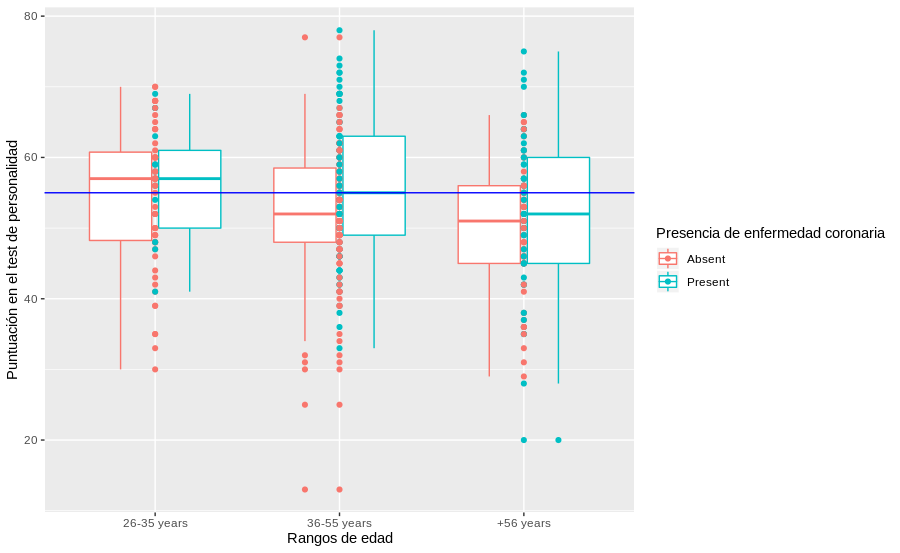
\includegraphics[scale=0.35]{images/question-4/plot2.png}
    \label{fig:question4-uplot1}
\end{wrapfigure}

Finalmente, en el grupo de las personas mayores de 55 años, no predomina la personalidad de tipo A, sino todo lo contrario. La personalidad en este rango de edad no es un factor tan relevante, pues aunque los pacientes con enfermedad coronaria superan a los que no la tienen (61 casos frente a 53), en el motivo para padecerla puede influir la edad, además de otras variables ocultas. \\

Cabe destacar que al categorizar la variable \texttt{typea} se está perdiendo información relevante que si aportaba la escala ordinal de valores del test. Para recuperar esta información, lo más adecuado es representar una gráfica de cajas como la de la derecha. En este diagrama se han representado las puntuaciones en el test de personalidad de tipo A, respecto a los rangos de edad. Se puede observar que en el intervalo de edad más significativo (entre 35 y 55 años), el valor en el test de personalidad es más importante cuando está presente la enfermedad, coincidiendo la mediana de las observaciones con el umbral que marca la presencia de comportamiento tipo A.

\vspace{5mm}

\section{Plan de Análisis de Datos}

\begin{figure}[H]
    \centering
    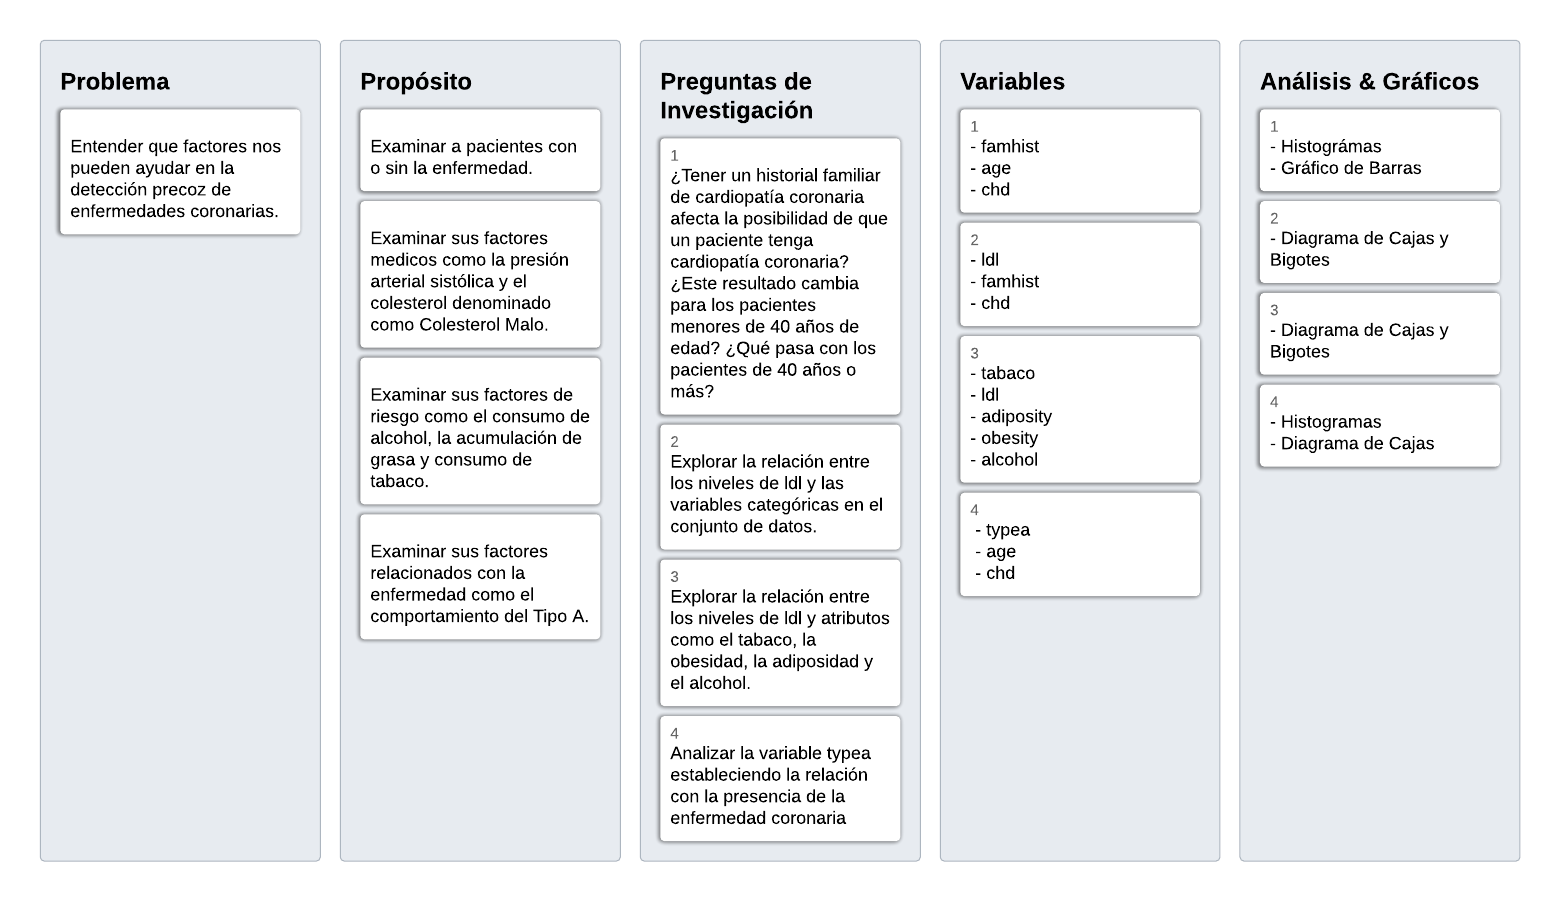
\includegraphics[scale=0.2]{images/data_analysis/plan.png}
    \label{image:data-ana}
\end{figure}

\vspace{3mm}

Tras haber seguido el plan de análisis de datos, llegamos a la conclusión de que para la consecución de un modelo que sepa predecir que pacientes son propensos a padecer enfermedades coronarias se necesitaría una recogida de información más extensa. Para, tras haber vuelto a analizar el nuevo dataset y haber hecho un preprocesamiento del mismo, entrenar un modelo de regresión lineal que cumpla el propósito propuesto dentro del Plan de Análisis de Datos.

\vspace{5mm}

\section{Conclusiones y Limitaciones de los Resultados}

Las conclusiones extraídas en este trabajo se corresponden con las conclusiones finales obtenidas para responder cada una de las preguntas. En la primera pregunta, se ha visto que el impacto del histórico familiar en la posibilidad de padecer o no una enfermedad coronaria se hace presente a partir \texttt{40} años e incrementa con la edad, por ello, el estudio de pacientes mayores de 40 años en una nueva recolección de información sería muy interesante de cara sobretodo a poder constatar este fenómeno. En las dos preguntas siguientes se ha estudiado la variable que determina el nivel de colesterol malo (\texttt{ldl}). 

\vspace{3mm}

En la segunda pregunta se ha constatado la importancia del historial familiar respecto a esta variable y en la siguiente pregunta se ha discriminado la relación directa con el alcohol y el tabaco pero demostrando la correlación entre adiposidad y obesidad, y de éstos con los niveles de colesterol malo, para los cuales, valores bajos de adiposity y obesity se traducen en valores reducidos de ldl. 

\vspace{3mm}

En la tercera pregunta se ha estudiado la relación de la personalidad con la presencia de enfermedades coronarias. Este análisis no ha revelado que realmente exista una relación directa, sin embargo, si que existe una predisposición a padecer la enfermedad en los pacientes con un rango de edad comprendido entre 35 y 55 años.

\vspace{3mm}

El análisis de este conjunto de datos nos ha permitido obtener diversas conclusiones, sin embargo, la mayor dificultad que nos hemos encontrado ha sido la poca cantidad y diversidad de los datos que poseemos. Este conjunto de datos tiene fines educativos, y por ello, no cuenta con toda la cantidad de datos y variables necesarias. Lo hemos considerado un conjunto de datos homogéneo, es decir, solo contamos con pacientes masculinos y de una localidad determinada, con poca diversidad en cuanto a rangos de edad y poca variedad en los consumos de tabaco y alcohol. Para poder continuar esta línea de trabajo es imprescindible aumentar o buscar un nuevo conjunto de datos.

\begin{thebibliography}{9}
\bibitem{bortner1969short}
    Journal of chronic diseases (Bortner, Rayman W)
    \newblock {\em A short rating scale as a potential measure of pattern A behavior}, 1969.

\end{thebibliography}

\end{document}



